\begin{figure*}[hbtp]
  \centering
  \subfigure[Speedup of \textit{DLH} approach with different hub limits $L_H$]{
    \label{fig:adjust-overall--runtime}
    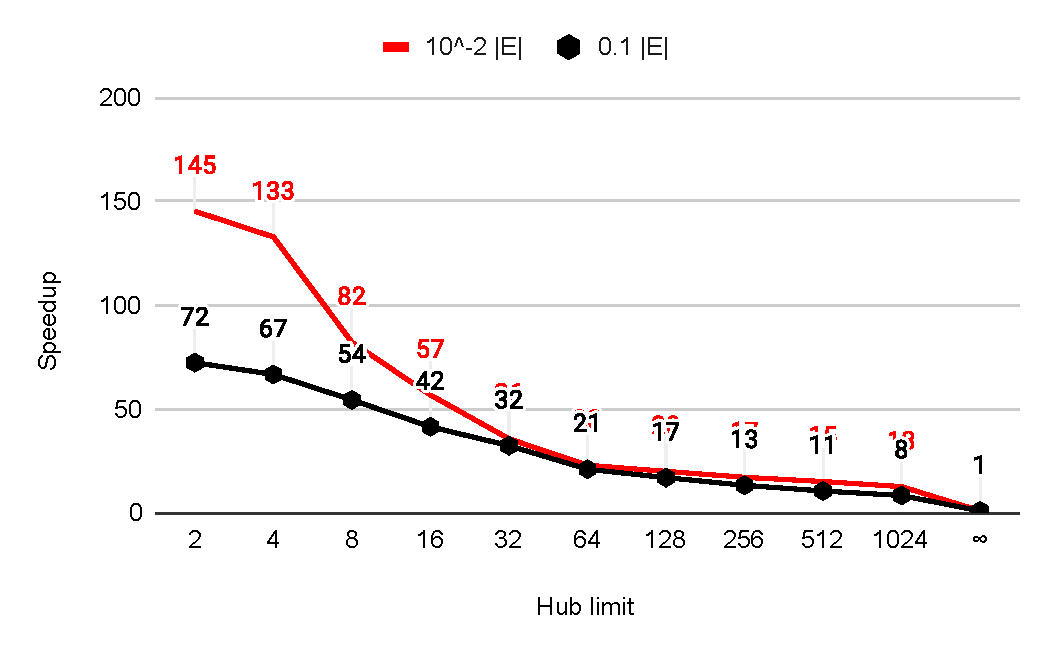
\includegraphics[width=0.48\linewidth]{out/adjust-overall-speedup.pdf}
  }
  \subfigure[F1 score of predicted links (logarithmic scale), with different hub limits $L_H$]{
    \label{fig:adjust-overall--precision}
    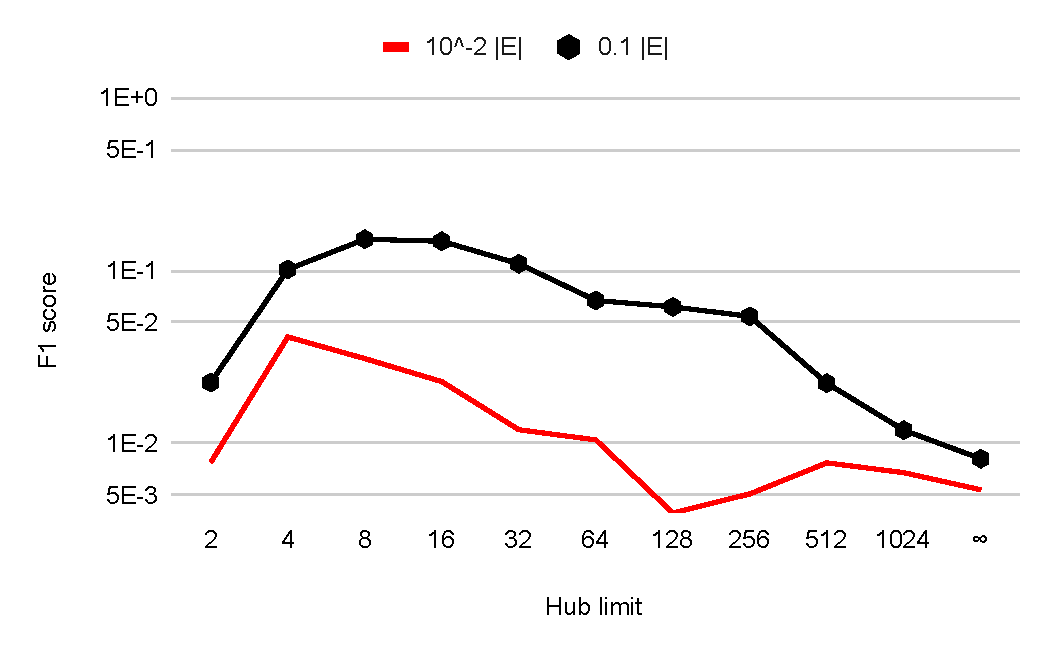
\includegraphics[width=0.48\linewidth]{out/adjust-overall-f1score.pdf}
  } \\[0ex]
  \caption{Overall impact of adjusting the hub limit $L_H$ from $2$ to $1024$ (in multiples of $2$), and to $\infty$, on the speedup and F1 score of predicted links (log scale), of neighbor-based link prediction methods, with the number of unobserved edges $E^U$ of $10^{-2}|E|$ and $0.1|E|$. Speedup is measured with respect to hub limit $L_H$ of $\infty$, i.e., the \textit{Improved Baseline (IBase)} approach.\ignore{, using geometric mean of runtimes for link prediction using the DLH approach using all similarity scores given in Section \ref{sec:metrics}; while overall F1 score is obtained by taking the average.}}
  \label{fig:adjust-overall}
\end{figure*}
